% Vorlesung 13.12.18 (11 Days until christmas)


% ab Hier auch richtige Phi und keine varPhis

\chapter{Zeitabhängige elektromagnetische Felder - Elektrodynamik}

bisher Zeitunabhängige Felder:
\begin{equation*}
\, \vabla \cdot \vec{D} = \rho \qquad \, \vabla \times \vec{E} = 0 \qquad \tx{Elektrostatik}
\end{equation*}
\begin{equation*}
\ \ \: \vabla \cdot \vec{B} = 0 \qquad \vabla \times \vec{H} = \vec{j} \qquad \tx{Magnetostatik}
\end{equation*}
Zeitabhängige Felder:
\begin{equation*}
\vec{B}(\vec{r}, t) \leftrightarrow \vec{E}(\vec{r}, t)
\end{equation*}

\section{Maxwell-Gleichungen}

\begin{align*}
\vabla \cdot \vec{D} &= \rho \qquad \, \vabla \times \vec{E} + \prt{\vec{B}}{t} = 0 \\
\vabla \cdot \vec{B} &= 0 \qquad \vabla \times \vec{H} - \prt{\vec{D}}{t} = \vec{j}
\end{align*}
$ \prt{\vec{B}}{t} \ $ ist die Induktion\\[3pt]
$ \prt{\vec{D}}{t} \ $ ist der Verschiebungsstrom\\

\subsection{Faraday'sches Induktionsgesetz}

\begin{equation*}
\vabla \times \vec{E} = - \prt{\vec{B}}{t}
\end{equation*}
\begin{center}
	%t1: %t2:
	\begin{tikzpicture}
	% \draw (0,0) ellipse (1cm and .7cm);
	\coordinate (r) at (-2.2,0);
	\draw[->] ($ ({cos(45) * -.9},{sin(45) * -.6}) + (r) $) arc[start angle=-135, end angle=225, x radius = .9cm, y radius = .6cm] node[anchor=north east] {$ \partial F $};
	\draw[->] ($ ({cos(45) * .9},{sin(45) * .6}) + (r) $) arc[start angle=-315, end angle=45, x radius = .9cm, y radius = .6cm];
	\node at (r) {$ F $};
	\node[left] at ($ (r) + (-1,0) $) {$ U_{\tx{ind}} $};
	\draw[fill=gray!30!white] (-.3,-.7) rectangle node[] {$ \substack{\tx{\Large{S}} \\[10pt] \tx{\Large{N}}} $} (.3,.7);
	\draw[->] (0,0) -- (.7,0) node[right] {$ \vec{v} $};
	
	\draw[looseness=2] (.15,.7) to[out=80,in=90] (1.2,0) to[out=-90,in=-80] (.15,-.7);
	\draw[looseness=2] (.09,.7) to[out=84,in=90] (1.8,0) to[out=-90,in=-84] (.09,-.7);
	\draw[looseness=2.5] (.03,.7) to[out=88,in=90] (2.6,0) to[out=-90,in=-88] (.03,-.7);
	
	\draw[looseness=2] (-.15,.7) to[out=100,in=90] (-1.2,0) to[out=-90,in=-100] (-.15,-.7);
	\draw[looseness=2] (-.09,.7) to[out=96,in=90] (-1.8,0) to[out=-90,in=-96] (-.09,-.7);
	\draw[looseness=2.5] (-.03,.7) to[out=92,in=90] (-2.6,0) to[out=-90,in=-92] (-.03,-.7);
	\end{tikzpicture}
\end{center}
\begin{align*}
\int_F \dd \vec{f} \cdot (\vec{\nabla} \times \vec{E}) &= - \int \dd \vec{f} \cdot \prt{\vec{B}}{t} \\
= \ub{\int_{\partial F} \dd \vec{r} \cdot \vec{E}}_{U_{\tx{ind}}} &= - \prd{}{t} \ub{\int_F \dd \vec{f} \cdot \vec{B}}_{\Phi_m (t)}
\end{align*}
$ \Phi_m(t) $ ist der Fluss des $ \vec{B} $-Feldes durch F
\begin{equation*}
U_{\tx{ind}} = - \prd{}{t} \int_F \dd \vec{f} \cdot \vec{B}
\end{equation*}
\emph{Bemerkung:}
\begin{enumerate}[i)]
	\item Vorzeichen-Strom
	\begin{center}
			%t3:
			\begin{tikzpicture}[scale=1.25]
				\coordinate (a) at (0,0);
				\draw[->] ($ ({cos(45) * -.9},{sin(45) * -.6}) + (a) $) arc[start angle=-135, end angle=225, x radius = .9cm, y radius = .6cm] node[anchor=north east] {$ \partial F $};
				\draw[->] ($ ({cos(45) * .9},{sin(45) * -.6}) + (a) $) arc[start angle=-45, end angle=315, x radius = .9cm, y radius = .6cm] node[anchor=north west] {$ \vec{j} $};
				\draw[thick,->] ($ (a) + (.3,-.3) $) -- ++(0,.6);
				\draw ($ (a) + (.4,0) $) -- ++(1,.5) node[right] {$ \vec{B}(t_1) = \vec{B}_1 $};
				\draw[thick,->] ($ (a) + (-.3,.3) $) -- node[left=10pt] {$ \dd \vec{f} $} ++(0,.6);
				
				\coordinate (b) at (6,0);
				\draw[->] ($ ({cos(45) * -.9},{sin(45) * -.6}) + (b) $) arc[start angle=-135, end angle=225, x radius = .9cm, y radius = .6cm] node[anchor=north east] {$ \partial F $};
				\draw[->] ($ ({cos(45) * .9},{sin(45) * -.6}) + (b) $) arc[start angle=-45, end angle=315, x radius = .9cm, y radius = .6cm] node[anchor=north west] {$ \vec{j} $};
				\draw[thick,->] ($ (b) + (.3,-.3) $) -- ++(0,.6);
				\draw ($ (b) + (.4,0) $) -- ++(1,.5) node[right] {$ \vec{B}(t_2) = \vec{B}_2 $};
				\draw[thick,->] ($ (b) + (-.3,.3) $) -- node[left=10pt] {$ \dd \vec{f} $} ++(0,.6);
			\end{tikzpicture}
	\end{center}
	\begin{equation*}
	t_2 > t_1 \qquad \vec{B}(t_1) > \vec{B}(t_2)
	\end{equation*}
	\begin{equation*}
	\Phi_m(t_1) = \int_F \dd \vec{f} \vec{B}_1 > \Phi_m(t_2) = \int_F \dd \vec{f} \vec{B}_2
	\end{equation*}
	\begin{equation*}
	\prd{}{t} \Phi_m(t) \le 0
	\end{equation*}
	\begin{equation*}
	\rightarrow \quad U_{\tx{ind}} = \int_{\partial F} \dd \vec{r} \cdot \vec{E} = - \prd{}{t} \Phi_m > 0
	\end{equation*}
	Mit $ \vec{j} = \sigma \vec{E} $, wobei $ \sigma $ die Leitfähigkeit des Leiters ist erhalten wir:
	\begin{equation*}
	\rightarrow \quad \int_{\partial F} \dd \vec{r} \cdot \vec{j} > 0 \qquad \rightarrow \quad \vec{j} \parallel \partial F
	\end{equation*}
	\begin{minipage}{.5\linewidth}
		$ \Rightarrow $ \textbf{Lenz'sche Regel:}\\
		Der induzierte Strom und das damit verbundene Magnetfeld sind so gerichtet, dass sie der Ursache ihrer Entstehung entgegenwirken.
	\end{minipage}%
	\begin{minipage}{.5\linewidth}
		\flushright
		%t4:
		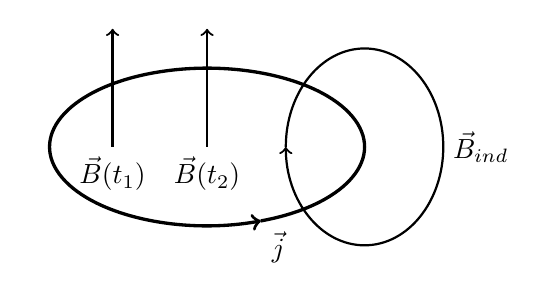
\begin{tikzpicture}
			\draw[->,very thick] ({cos(70) * 2cm}, {sin(70) * -1cm}) arc[start angle=-70, end angle=290,x radius = 2cm, y radius = 1cm] node[anchor=north west] {$ \vec{j} $};
			\draw[->, thick] (1,0) arc[start angle=180,end angle=-180,x radius=1cm, y radius=1.25cm];
			\node[right] at (3,0) {$ \vec{B}_{\tx{ind}} $};
			\foreach \x\n in {-1.2/1,0/2}
			\draw[thick,->] (\x,0) node[below] {$ \vec{B}(t_{\n}) $} -- ++(0,1.5);
		\end{tikzpicture}
	\end{minipage}%
	\item $ \Phi_m $ hängt nicht von der speziellen Form der Fläche $ F $ ab, sondern nur vom Rand $ \partial F $.\\
	\begin{center}
		%t5:
		\begin{tikzpicture}
			\coordinate (c1) at (0,0);
			\draw[fill=blue!30!white,->] ($ (c1) + ({sin(45) * 1cm},{cos(45) * -.5cm}) $) arc[start angle=-45, end angle=315, x radius=1cm, y radius=.5cm] node[anchor=north west] {$ \partial F $};
			\draw[->] ($ (c1) + (.25,.25) $)  -- node[right] {$ \dd\vec{f}_1 $} ++(0,1);
			
			\coordinate (c2) at (4,0);
			\draw[fill=red!30!white,looseness=2] ($ (c2) + (-1,0) $) to[out=-90,in=-90] ($ (c2) + (1,0) $);
			\draw[fill=red!13!white,->] ($ (c2) + ({sin(45) * 1cm},{cos(45) * -.5cm}) $) arc[start angle=-45, end angle=315, x radius=1cm, y radius=.5cm] node[xshift=.7cm] {$ \partial F $};
			\draw[->] ($ (c2) + (.25,-.3) $)  -- node[right,yshift=10pt] {$ \dd\vec{f}_2 $} ++(0,1.55);
			\draw ($ (c2) + (.6,-.8) $) to[out=-50,in=200] ++(1,-.2) node[right] {$ F_2 $};
			\node at ($ (c2) + (3.5,0) $) {$ \Phi_1 = \Phi_2 $};
			
			\coordinate (c3) at (2,-3);
			\draw[fill=red!30!white,looseness=2] ($ (c3) + (-1,0) $) to[out=-90,in=-90] ($ (c3) + (1,0) $);
			\draw[fill=blue!30!white] ($ (c3) + ({sin(45) * 1cm},{cos(45) * -.5cm}) $) arc[start angle=-45, end angle=315, x radius=1cm, y radius=.5cm];
			\draw[->] ($ (c3) + (-.25,.25) $)  -- node[left=5pt] {$ \dd\vec{f}_1 $} ++(0,1);
			\draw[->] ($ (c3) + (.25,-.75) $) -- node[right=5pt] {$ - \dd \vec{f_2} $} ++(0,-1);
		\end{tikzpicture}
	\end{center}
	
	\noindent
	Aus der Skizze und mit Satz von Gauß. (Der Fluss durch eine geschlossene Fläche ist gleich 0):
	\begin{equation*}
	\Phi = \int_F \dd \vec{f} \cdot \vec{B} = 0
	\end{equation*}
	\begin{equation*}
	\Phi_{\tx{m}_1} = \Phi_{\tx{m}_2}
	\end{equation*}
	\begin{equation*}
	0 = \int_F \dd \vec{f} \cdot \vec{B} = \ub{\int_{F_1} \dd \vec{f}_1 \cdot \vec{B}}_{\Phi_{\tx{m}_1}} - \ub{\int_{F_2} \dd \vec{f}_2 \cdot \vec{B}}_{\Phi_{\tx{m}_2}}
	\end{equation*}
	\item Eine Flussänderung kann auf verschiedene Weise zustandekommen:\\
	\begin{minipage}{.5\linewidth}
		\begin{itemize}
			\item Veränderung des Magnetfeldes $ \vec{B}(t) $
			\item Bewegung der Leiterschleife im äußeren Feld
		\end{itemize}
		\vspace{40pt}
	\end{minipage}%
	\begin{minipage}{.5\linewidth}
		\begin{center}
			%t6:
			\begin{tikzpicture}[scale=.8]
				\coordinate (r) at (-2.2,0);
				\draw[thick,->] ($ ({cos(45) * -.9},{sin(45) * -.6}) + (r) $) arc[start angle=-135, end angle=225, x radius = .9cm, y radius = .6cm];
				\draw[fill=gray!30!white] (-.3,-.7) rectangle node[] {$ \substack{\tx{\Large{S}} \\[10pt] \tx{\Large{N}}} $} (.3,.7);
				\draw[thick,->] (0,0) -- (1.1,0) node[right] {$ \vec{v} $};
				\draw[thick,->] ($ (r) + (-1,0) $) -- ++(-1.1,0);
				
				\draw[looseness=2] (.15,.7) to[out=80,in=90] (1.2,0) to[out=-90,in=-80] (.15,-.7);
				\draw[looseness=2] (.09,.7) to[out=84,in=90] (1.8,0) to[out=-90,in=-84] (.09,-.7);
				\draw[looseness=2.5] (.03,.7) to[out=88,in=90] (2.6,0) to[out=-90,in=-88] (.03,-.7);
				
				\draw[looseness=2] (-.15,.7) to[out=100,in=90] (-1.2,0) to[out=-90,in=-100] (-.15,-.7);
				\draw[looseness=2] (-.09,.7) to[out=96,in=90] (-1.8,0) to[out=-90,in=-96] (-.09,-.7);
				\draw[looseness=2.5] (-.03,.7) to[out=92,in=90] (-2.6,0) to[out=-90,in=-92] (-.03,-.7);
			\end{tikzpicture}
		\end{center}
	\end{minipage}%
\end{enumerate}
\begin{equation*}
\vabla \times \vec{E} = - \prt{\vec{B}}{t}
\end{equation*}
Ein zeitlich verändertes $ \vec{B} $-Feld erzeugt ein elektrisches Wirbelfeld analog zu:
\begin{equation*}
\vabla \times \vec{B} = \mu_0 \vec{j}
\end{equation*}
\begin{center}
	%t7:
	\begin{tikzpicture}
		\draw[very thick, ->] (0,-1) -- (0,1) node[left] {$ \vec{j} $};
		\draw[->] ({.5 * sin(45)},-{.25 * cos(45)}) arc[start angle=-45,end angle=315, x radius=.5, y radius=.25];
		\draw[->] ({1 * sin(45)},-{.5 * cos(45)}) arc[start angle=-45, end angle=315, x radius=1, y radius=.5];
		\node at (.7,-.7) {$ \vec{B} $};
		
		\coordinate (a) at (3,0);
		\draw[very thick, ->] ($ (a) + (-.175,-1) $) -- ++(0,2);
		\draw[very thick, ->] ($ (a) + (.175,-1) $) -- ++(0,2);
		\draw[->] ($ (a) + ({.5 * sin(45)},-{.25 * cos(45)}) $) arc[start angle=-45,end angle=315, x radius=.5, y radius=.25];
		\draw[->] ($ (a) + ({1 * sin(45)},-{.5 * cos(45)}) $) arc[start angle=-45, end angle=315, x radius=1, y radius=.5];
		\node at ($ (a) + (1,-1) $) {$ \prt{\vec{B}}{t} $};
	\end{tikzpicture}
\end{center}

\subsection{Maxwellscher Verschiebungsstrom}

Magnetostatik:
\begin{equation*}
\vabla \times \vec{H} = \vec{j} \qquad \tx{Ampere}
\end{equation*}
Dies kann in der Elektrodynamik nicht gelten, dies zeigen wir indem wir auf beiden Seiten die Divergenz bilden.
\begin{equation*}
\ub{\vabla \cdot (\vabla \times \vec{H})}_{=0} = \vabla \cdot \vec{j} \quad \Rightarrow \quad \vabla \cdot \vec{j} = 0 \quad \tx{bei stationären Strömen}
\end{equation*}
im Allgemeinen haben wir zeitlich abhängige Ströme:
\begin{equation*}
\vabla \cdot \vec{j}(\vec{r},t) \overset{\tx{i.A.}}{\neq} 0
\end{equation*}
Kontinuitätsgleichung:
\begin{equation*}
\prt{\rho}{t} + \vabla \cdot \vec{j} = 0
\end{equation*}
Ergänzung:
\begin{equation*}
\vabla \times \vec{H} = \vec{j} + \vec{j}_0
\end{equation*}
\begin{equation*}
\Rightarrow \quad \ub{\vabla \cdot (\vabla \times \vec{H})}_{= 0} = \ub{\vabla \cdot \vec{j}}_{= - \prt{\rho}{t}} + \vabla \cdot \vec{j}_0
\end{equation*}
\begin{equation*}
\Rightarrow \quad \vabla \cdot \vec{j}_0 = \prt{\rho}{t} = \prt{}{t} \vabla \cdot \vec{D} = \vabla \cdot \left(\prt{\vec{D}}{t}\right)
\end{equation*}
\begin{equation*}
\rightarrow \quad \vec{j}_0 = \prt{\vec{D}}{t}
\end{equation*}
Damit erhalten wir für die die Stromdichte:
\begin{equation*}
\vabla \times \vec{H} - \prt{\vec{D}}{t} = \vec{j}
\end{equation*}
\emph{Beispiel:} \textbf{Plattenkondensator}\\
\begin{minipage}{.6\linewidth}
	\begin{equation*}
	\vec{D} = \casess{\sigma \vec{e}_x}{\tx{innen}}{0}{\tx{außen}}
	\end{equation*}
	$ \sigma = \frac{1}{F} $
	\begin{equation*}
	\prt{\vec{D}}{t} = \frac{\vec{e}_x}{F} \equalto{\prd{q}{t}}{I} = \frac{I}{F} \vec{e}_x
	\end{equation*}
	\begin{equation*}
	\vabla \times \vec{H} - \prt{\vec{D}}{t} = \vec{j}
	\end{equation*}
	innen: $ \vec{j} = 0 $
	\begin{equation*}
	\vabla \times \vec{H} = \prt{\vec{D}}{t} =  \frac{I}{F} \vec{e}_x
	\end{equation*}
\end{minipage}%
\begin{minipage}{.4\linewidth}
	\flushright
	%t8:
	\begin{tikzpicture}[scale=1]
		\draw[very thick] (-1.5,-2) -- (-1.5,2) node[above] {$ q $};
		\draw[very thick] (1.5,-2) -- (1.5,2) node[above] {$ - q $};
		
		\foreach \y in {-1.8,-.6,.6,1.8}
		\draw[->] (-1.3,\y) -- (1.3,\y);
		
		\foreach \y in {-1.8,-.6,.6,1.8}
		\draw[fill = white!20!red] (-1.8,\y) circle (.2cm) node[] {$ \color{white} + \color{white} $};
		
		\foreach \y in {-1.8,-.6,.6,1.8}
		\draw[fill = white!20!blue] (1.8,\y) circle (.2cm) node[] {$ \color{white} - \color{white} $};
		
		\node at (0,1.2) {$ \vec{D} $};
		\node at (0,-1.2) {$ \vec{H} $};
		
		\draw[->] (0,-3) -- ++(1.5,0) node[right] {$ x $};
		\draw (0,-3.1) -- (0,-2.9);
		
		\draw[very thick] (-1.5,-2) -- (-1.5,-2.5);
		\draw[very thick] (1.5,-2) -- (1.5,-2.5);
		\draw[->] (-1.5,-2.5) -| (-3,-4) -- (0,-4) node[below] {\Large{$ I $}};
		\draw (1.5,-2.5) -| (3,-4) -- (0,-4);
		\draw[thick,->] ($ (-2.5,-2.5) + ({sin(45) * .3},{cos(45) * -.8}) $) arc[start angle=-45, end angle=315, x radius=.3, y radius=.8];
		\draw[thick,->] ($ (2.5,-2.5) + ({sin(45) * .3},{cos(45) * -.8}) $) arc[start angle=-45, end angle=315, x radius=.3, y radius=.8];
	\end{tikzpicture}
\end{minipage}%

\subsection{Lösung der Differentialgleichungen} %check this

\begin{align*}
\vabla \cdot \vec{D} &= \rho \qquad \, \vabla \times \vec{E} + \prt{\vec{B}}{t} = 0 \\
\vabla \cdot \vec{B} &= 0 \qquad \vabla \times \vec{H} - \prt{\vec{D}}{t} = \vec{j}
\end{align*}
Zwei homogene und zwei inhomogene Differentialgleichungen. Zur Lösung benötigt man also zusätzliche Materialgleichungen:
\begin{equation*}
\vec{B} = \mu_0 (\vec{H} + \vec{M}) \qquad \vec{D} = \epsilon_0\vec{E} + \vec{P}
\end{equation*}
bei linearen Medien:
\begin{equation*}
\vec{B} = \mu \vec{H} \qquad \vec{D} = \epsilon \vec{E}
\end{equation*}
Die Kraft ist:
\begin{equation*}
\vec{F} = q (\vec{E} + \vec{v} \times \vec{B})
\end{equation*}
\textbf{Intagrale Form der Maxwell-Gleichungen}
\begin{align*}
\oint_F \dd \vec{f} \cdot \vec{B} &= 0  \qquad \qquad \qquad \int_{\partial F} \dd \vec{r} \cdot \vec{E} + \prd{}{t} \int_F \dd \vec{f} \cdot \vec{B} = 0 \\
\int_{\partial V} \dd \vec{f} \cdot \vec{D} &= \int_V \dd^3 r \rho(\vec{r}) \quad \ \ \int_{\partial F} \dd \vec{r} \cdot \vec{H} - \prd{}{t} \int_F \dd \vec{f} \cdot \vec{D} = \int_F \dd \vec{f} \cdot \vec{j}
\end{align*}
\textbf{Mikroskopische Maxwell-Gleichungen:}\\
formal:
\begin{equation*}
\vec{D} = \epsilon_0 \vec{E} \qquad \vec{H} = \frac{1}{\mu_0} \vec{B}
\end{equation*}
\begin{align*}
\vabla \cdot \vec{B} &= 0 \qquad \quad \vabla \times \vec{E} + \prt{\vec{B}}{t} = 0\\
\vabla \cdot \vec{E} &= \frac{1}{\epsilon_0} \rho \qquad \vabla \times \vec{B} - \epsilon_0 \mu_0 \prt{\vec{E}}{t} = \mu_0 \vec{j}
\end{align*}

\section{Potentiale der Elektrodynamik - Eichtransformation}

\begin{equation*}
\vabla \cdot \vec{B} = 0 \qquad \vec{B}(\vec{r},t) = \vabla \times \vec{A}(\vec{r},t)
\end{equation*}
\begin{align*}
\vabla \times \vec{E} + \prt{\vec{B}}{t} = 0 \qquad 0 &= \vabla \times \vec{E} + \prt{}{t} \vabla \times \vec{A} \\
&= \vabla \times \left(\vec{E} + \prt{\vec{A}}{t}\right)
\end{align*}
\begin{equation*}
\Rightarrow \quad \vec{E} + \prt{\vec{A}}{t} = - \vabla \Phi
\end{equation*}
$ \Phi $ ist ein skalares Potential
\begin{equation*}
\Rightarrow \quad \vec{E}(\vec{r},t) = - \vabla \Phi(\vec{r},t) - \prt{\vec{A}(\vec{r},t)}{t}
\end{equation*}
Damit haben wir die beiden homogenen Gleichungen gelöst. Wir können $ \vec{E} $- und $ \vec{B} $-Felder nun durch die Potentiale $ \Phi $ und $ \vec{A} $ ausdrücken.

\subsection{Bestimmungsgleichung für \texorpdfstring{$ \Phi , \vec{A} $}{phi A}}

\begin{equation*}
\vec{D} = \epsilon \vec{E} \qquad \vec{H} = \frac{1}{\mu} \vec{B}
\end{equation*}
\begin{align*}
\rightarrow \quad &\vabla \cdot \vec{E} = \frac{1}{\epsilon} \rho \\
& \vabla \times \vec{B} - \epsilon \mu \prt{\vec{E}}{t} = \mu \vec{j}
\end{align*}
\begin{equation*}
\frac{1}{\epsilon} \rho = \vabla \cdot \left(- \vabla \Phi - \prt{\vec{A}}{t}\right) = - \Delta \Phi - \prt{}{t} \vabla \cdot \vec{A}
\end{equation*}
\begin{equation*}
\rmbox{\Rightarrow \quad \Delta \Phi + \prt{}{t} \vabla \cdot \vec{A} = - \frac{1}{\epsilon} \rho}
\end{equation*}
\begin{equation*}
\mu \vec{j} = \ub{\vabla \times (\vabla \times \vec{A})}_{=\vabla \cdot (\vabla \cdot \vec{A}) - \Delta \vec{A}} - \epsilon \mu \prt{}{t} \left(- \vabla \Phi - \prt{\vec{A}}{t}\right)
\end{equation*}
\begin{equation*}
\rmbox{\Rightarrow \quad \Delta \vec{A} - \epsilon \mu \prt{^2 \vec{A}}{t^2} - \vabla \cdot \left(\vabla \cdot \vec{A} + \epsilon \mu \prt{\Phi}{t}\right) = - \mu \vec{j}}
\end{equation*}

\subsection{Eichtransformation}

$ \Phi, \vec{A} $ sind durch:
\begin{equation*}
\vec{B} = \vabla \times \vec{A} \qquad \vec{E} = - \vabla \Phi - \prt{\vec{A}}{t}
\end{equation*}
nicht eindeutig festgelegt.\\[5pt]
\textbf{Eichtransformation:}
\begin{align*}
\vec{A}'(\vec{r},t) &= \vec{A}(\vec{r},t) + \vabla \Lambda(\vec{r},t)\\
\Phi'(\vec{r},t) &= \Phi(\vec{r},t) - \prt{\Lambda(\vec{r},t)}{t}
\end{align*}
\begin{equation*}
\vabla \times \vec{A}' = \vabla \times \vec{A} + \ub{ \vabla (\vabla \Lambda)}_{=0} = \vabla \times \vec{A} = \vec{B} \quad \checkmark
\end{equation*}
\begin{equation*}
- \vabla \Phi' - \prt{\vec{A}'}{t} = - \vabla \Phi + \cancel{\vabla \prt{\Lambda}{t}} - \prt{\vec{A}}{t} - \cancel{\prt{}{t} \vabla \Lambda} = \vec{E} \quad \checkmark 
\end{equation*}
$ \rightarrow $ verschiedene Eichungen.
\begin{enumerate}[1)]
	\item \textbf{Coulomb-Eichung}
	\begin{equation*}
	\vabla \cdot \vec{A}(\vec{r},t) = 0
	\end{equation*}
	\begin{equation*}
	\rmbox{\rightarrow \quad \Delta \Phi(\vec{r},t) = - \frac{1}{\epsilon} \rho(\vec{r},t)}
	\end{equation*}
	\begin{equation*}
	\Phi(\vec{r},t) = \frac{1}{4 \pi \epsilon} \int \dd ^3 r' \frac{\rho(\vec{r}',t)}{|\vec{r} - \vec{r}'|}
	\end{equation*}
	\begin{equation*}
	\rmbox{ \rightarrow \quad \Delta \vec{A} - \epsilon \mu \prt{^2 \vec{A}}{t^2} = \mu \vec{j} + \epsilon \mu \vabla \prt{\Phi}{t}}
	\end{equation*}
	Typische Anwendung:\\
	Bei statischen Problemen und bei nicht relativistischen Geschwindigkeiten.\\
	Die Coulomb-Eichung ist nicht Lorenz-invariant.
	\item \textbf{Lorenz-Eichung}
	\begin{equation*}
	\vabla \cdot \vec{A} + \epsilon \mu \prt{\Phi}{t} = 0
	\end{equation*}
	Im Vakuum: $ \epsilon \mu = \epsilon_0 \mu_0 = \frac{1}{c^2} $
	\begin{equation*}
	\rightarrow \quad \Delta \Phi + \prt{}{t} \left(- \epsilon \mu \prt{\Phi}{t}\right) = 0
	\end{equation*}
	\begin{equation*}
	\rmbox{\rightarrow \quad \Delta \Phi - \epsilon \mu \prt{^2 \Phi}{t^2} = 0 \ / \ - \frac{1}{\epsilon} \rho}
	\end{equation*}
	\begin{equation*}
	\rmbox{\rightarrow \quad \Delta \vec{A} - \epsilon \mu \prt{^2 \vec{A}}{t^2} = 0 \ / \ \mu_0 \vec{j} \ \ }
	\end{equation*}
\end{enumerate}

% Vorlesung 17.12.18 (7 Days until Christmas)

\section{Energie und Impuls elektromagnetischer Felder}

\subsection{Energie des EM-Feldes}

\begin{minipage}{.7\linewidth}
	System von Punktladungen $ q_i, m_i, \vec{r}_i, \vec{v}_i $ im Volumen $ V $:\\[5pt]
	Kraft auf Ladungen im elektromagnetischen Feld:
	\begin{equation*}
	\vec{F}_i = q_i \left(\vec{E}(\vec{r}_i, t) + \vec{r}_i \times \vec{B}(\vec{r}_i, t) \right)
	\end{equation*}
\end{minipage}%
\begin{minipage}{.3\linewidth}
	%t1:
	\centering
	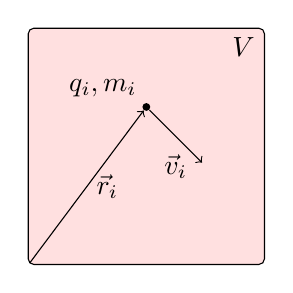
\begin{tikzpicture}
		\draw[fill=red!12!white,rounded corners=2pt] (0,0) rectangle (3,3);
		\node[fill=black,circle,inner sep=1pt, minimum size=1pt] (a) at (1.5,2) {};
		\draw[->] (0.02,0.02) -- node[right] {$ \vec{r}_i $} (a);
		\draw[->] (a) -- node[below=3pt] {$ \vec{v}_i $} ++(-45:1cm);
		\node[anchor=south east] at (a) {$q_i, m_i$};
		\node[anchor=north east] at (3,3) {$ V $};
	\end{tikzpicture}
	\vspace{5pt}
\end{minipage}%
\\
Zeitliche Änderung der Energie der Punktladungen durch die elektromagnetischen Felder:
\begin{align*}
\prd{}{t} W_{\tx{mat}} &= \prd{}{t} \sum_i \frac{m_i}{2} \vec{v}_i^2 = \sum_i \vec{v}_i \cdot \prd{\vec{v}_i}{t} = \sum_i \vec{v}_i \cdot \vec{F}_i\\
&= \sum_i q_i \vec{v}_i \cdot \vec{E}(\vec{r}_i, t) + \sum_i q_i \ub{ \vec{v}_i \cdot (\vec{v}_i) \times \vec{B}(\vec{r}_i, t) }_{=0}\\
&= \sum_i q_i \vec{v}_i \cdot \vec{E}(\vec{r}_i, t)
\end{align*}
formale Kontinuierliche Beschreibung: $ \vec{j}(\vec{r},t) = \sum_i q_i \vec{r}_i \delta(\vec{r} - \vec{r}_i(t)) $
\begin{equation*}
\rightarrow \quad \prd{}{t} W_{\tx{mat}} = \int_V \dd^3 r \ \vec{j}(\vec{r},t) \cdot \vec{E}(\vec{r},t)
\end{equation*}
Energiedichte $ w_{\tx{mat}} $: $ W_{\tx{mat}} = \int_V \dd^3 r \ w_{\tx{mat}} (\vec{r}) $
\begin{equation*}
\Rightarrow \quad \int_V \dd^3 r \ \vec{j} \cdot \vec{E} = \prd{}{t} \int_V \dd^3 r \ w_{\tx{mat}} = \int_V \dd^3 r \ \prt{}{t} w_{\tx{mat}}
\end{equation*}
\begin{equation*}
\Rightarrow \quad \int_V \dd^3 r \ \left(\prt{w_{\tx{mat}}}{t} - \vec{j} \cdot \vec{E} \right) = 0 \qquad \forall \ V
\end{equation*}
\begin{equation*}
\Rightarrow \quad \prt{w_{\tx{mat}}}{t} = \vec{j} \cdot \vec{E} \quad \widehat{=} \quad \tx{Leistungsdichte}
\end{equation*}
\begin{equation*}
[\vec{j}] [\vec{E}] = \frac{\tx{A}}{\tx{m}^2} \frac{\tx{V}}{\tx{m}} = \frac{\tx{W}}{\tx{m}^2}
\end{equation*}
Die gesamte Änderung der Energie der Materie im Volumen $ V $ ist dann:
\begin{equation*}
\prd{}{t} W_{\tx{mat}_V} = \int_V \dd^3 r \ \vec{j} \cdot \vec{E}
\end{equation*}
Außerdem gilt auch:
\begin{equation*}
\prd{}{t} W_{\tx{mat}} = - \prd{}{t} W_{\tx{feld}}
\end{equation*}
Wir wollen nun $ \vec{j} $ ersetzen und nutzen:
\begin{equation*}
\vec{j} = \vabla \times \vec{H} - \prt{\vec{D}}{t} \quad \Rightarrow \quad \vec{j} \cdot \vec{E} = \vec{E} \cdot (\vabla \times \vec{H}) - \vec{E} \cdot \prt{\vec{D}}{t}
\end{equation*}
$ \vec{E} $ mal der Rotation von $ \vec{H} $ können wir umformen als:
\begin{equation*}
\vabla \cdot (\vec{E} \times \vec{H}) = \vec{H} \cdot \ub{(\vabla \times \vec{E})}_{- \prt{\vec{B}}{t}} - \vec{E} (\vabla \times \vec{H})
\end{equation*}
\begin{equation*}
\rightarrow \quad  \vec{j} \cdot \vec{E} = - \vec{H} \cdot \prt{\vec{B}}{t} - \vec{E} \cdot \prt{\vec{D}}{t} - \vabla \cdot (\vec{E} \times \vec{H}) = \prt{}{t} w_{\tx{mat}}
\end{equation*}
\begin{equation*}
\Rightarrow \quad \prd{}{t} W_{\tx{mat}_V} = - \int_V \dd^3 r \ \left(\vec{H} \cdot \prt{\vec{B}}{t} + \vec{E} \cdot \prt{\vec{D}}{t} \right) - \int_V \dd^3 r \ \vabla \cdot (\vec{E} \times \vec{H}) = - \prd{}{t} W_{\tx{feld}}
\end{equation*}
Zur Vereinfachung und Interpretation: $ \vec{H} = \frac{1}{\mu} \vec{B} \quad \vec{D} = \epsilon \vec{E} \quad \epsilon, \mu \const $
\begin{equation*}
\vec{H} \cdot \prt{\vec{B}}{t} = \frac{1}{\mu} \vec{B} \cdot \prt{\vec{B}}{t} = \frac{1}{2} \frac{1}{\mu} \prt{}{t} (\vec{B} \cdot \vec{B}) = \frac{1}{2} \prt{}{t} (\vec{H} \cdot \vec{B})
\end{equation*}
\begin{equation*}
\vec{E} \cdot \prt{\vec{D}}{t} = \epsilon \vec{E} \cdot \prt{\vec{E}}{t} = \frac{\epsilon}{2} \prt{}{t} (\vec{E} \cdot \vec{E}) = \frac{1}{2} \prt{}{t} (\vec{E} \cdot \vec{D})
\end{equation*}
\begin{equation*}
\prd{}{t} W_{\tx{mat}_V} = - \prd{}{t} \frac{1}{2} \int_V \dd^3r \ (\vec{H} \cdot \vec{B} + \vec{E} \cdot \vec{D}) - \int_V \dd^3r \ \vabla \cdot (\vec{E} \times \vec{H})
\end{equation*}
\textbf{Elektrostatik:}
\begin{equation*}
w_{\tx{el}} = \frac{\epsilon_0}{2} \vec{E}^2 \quad (\tx{Vakuum}) \qquad w_{\tx{el}} = \frac{1}{2} \vec{E} \cdot \vec{D} \quad (\tx{Medium})
\end{equation*}
\textbf{Magnetostatik:}
\begin{equation*}
w_{\tx{mag}} = \frac{1}{2 \mu_0} \vec{B}^2 \quad (\tx{Vakuum}) \qquad w_{\tx{mag}} = \frac{1}{2} \vec{H} \cdot \vec{B} \quad (\tx{Medium})
\end{equation*}
Energie des elektromagnetischen Feldes:
\begin{equation*}
\frac{1}{2} \int_V \dd^3 r \ (\vec{H} \cdot \vec{B} + \vec{E} \cdot \vec{D}) = W_{\tx{em}_V}
\end{equation*}
Energiedichte:
\begin{equation*}
w_{\tx{em}} = \frac{1}{2} (\vec{H} \cdot \vec{B} + \vec{E} \cdot \vec{D})
\end{equation*}
\begin{equation*}
\prd{}{t} W_{\tx{mat}_V} = - \prd{}{t} W_{\tx{em}_V} - \ub{\int_V \dd^3 r \ \vabla \cdot (\vec{E} \times \vec{H})}_{\mathclap{\substack{\tx{Energie, die aus } V \\ \tx{abfließt (Strahlung)}}}}
\end{equation*}
\begin{equation*}
\vec{S}(\vec{r},t) = \vec{E} \times \vec{H} \qquad \tx{\textbf{Pointing-Vektor}}
\end{equation*}
\begin{equation*}
\int_V \dd^3 r \ \vabla \vec{S} = \int_{\partial V} \dd\vec{f}  \cdot \vec{S}
\end{equation*}
\begin{equation*}
[\vec{S}] = [\vec{E}] [\vec{H}] = \frac{\tx{V}}{\tx{m}} \frac{\tx{A}}{\tx{m}} = \frac{\tx{W}}{\tx{m}^2} = \frac{\tx{J}}{\tx{m}^2 \tx{s}} = \frac{\tx{Energie}}{\tx{Fläche } \cdot \tx{ Zeit}}
\end{equation*}
$ \vec{S}: $ \textbf{Energiestromdichte}\\
\begin{minipage}{.8\linewidth}
	% Hier fehlt ein Text von Kim:
	$$ \int_{\partial V} \dd \vec{f} \cdot \vec{S} $$
	Energiestrom des EM-Feldes durch die Fläche $ \partial V $.
\end{minipage}%
\begin{minipage}{.2\linewidth}
	\flushright
	%t2:
	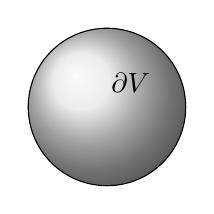
\begin{tikzpicture}
	\draw[shade, ball color=gray!20!white] (0,0) circle (1cm);
	\node at (.3,.3) {$ \partial V $};
	\end{tikzpicture}
\end{minipage}%

\subsubsection{Energiebilanz}

\begin{equation*}
\ub{\prd{}{t} W_{\tx{mat} _V}}_{\mathclap{\substack{\tx{an Ladungen} \\ \tx{in } V \tx{ verrichtete} \\ \tx{Arbeit}}}} \ \ + \ \ \ub{\prd{}{t} W_{\tx{em}_V}}_{\mathclap{\substack{\tx{Änderung der} \\ \tx{EM Feldenergie} \\ \tx{in } V}}} \ = \ \ub{- \int_{\partial V} \dd \vec{f} \cdot \vec{S}}_{\mathclap{\substack{\tx{Fluss der EM} \\ \tx{Feldenergie aus } V}}}
\end{equation*}
\emph{Bemerkung:}
\begin{enumerate}[i)]
	\item abgeschlossenes System (ohne Energiestromdichte ach außen) z.B. $ \mathbb{R}^3 $
	\begin{equation*}
	\int_V \dd \vec{f} \cdot \vec{S} \rightarrow 0
	\end{equation*}
	\item Gebiet ohne Ladungen und Ströme $ \rho = \vec{j} = 0 \ \ \tx{in} V $. $ w_{\tx{mat}} = \vec{j} \cdot \vec{E} = 0 $
	\begin{equation*}
	\prd{}{t} W_{\tx{mat}_V} = - \int_{\partial V} \dd \vec{f} \cdot \vec{S}
	\end{equation*}
	\item differentielle Form:
	\begin{equation*}
	\int_V \dd^3 r \ \left[\prt{w_{\tx{em}}}{t} + \vabla \cdot \vec{S} + \vec{j} \cdot \vec{E}\right] = 0
	\end{equation*}
	\frbox{Poyntigsches Theorem}{
	\begin{equation*}
	\rightarrow \quad \prt{w_{\tx{em}}}{t} + \prt{w_{\tx{mat}}}{t} + \vabla \cdot \vec{S} = 0
	\end{equation*}}
	oder auch: \textbf{Kontinuitätsgleichung für Energie}
	\begin{equation*}
	\prt{}{t} w + \vabla \cdot \vec{S} = 0
	\end{equation*}
	Analogie:
	\begin{equation*}
	\prt{\rho}{t} + \vabla \cdot \vec{j} = 0
	\end{equation*}
	\item \textbf{Poynting-Vektor}
	\begin{equation*}
	\vec{S} = \vec{E} \times \vec{H} \quad \tx{Energiestromdichte}
	\end{equation*}
	\textbf{Beachte:} Nur $ \vabla \cdot \vec{S} $ oder $ \int_{\partial V} \dd \vec{f} \cdot \vec{S} $ haben physikalische Bedeutung.\\[5pt]
	$ \vec{S} \to \vec{S} + \vabla \times \vec{G} $\\
	$ \vec{S} \neq 0 $, aber kein Energiestrom:
	\begin{equation*}
	\vec{E} = E \vec{e}_x \quad \vec{H} = H \vec{e}_y \qquad E,H \const
	\end{equation*}
	\begin{equation*}
	\vec{S} = \vec{E} \times \vec{H} = E H \vec{e}_z \neq 0
	\end{equation*}
	aber: $ \vabla \cdot \vec{S} = 0  \quad \rightarrow $ \textbf{kein Beitrag !}
\end{enumerate}
\emph{Beispiel:} \textbf{Energietransport in el./mag. Wellen im Vakuum}
\begin{center}
	%t3:
	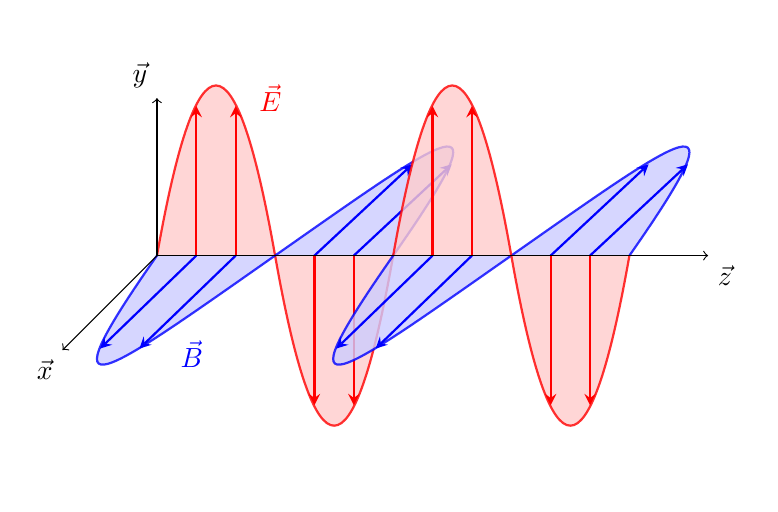
\begin{tikzpicture}%[>=stealth]
		% E
		\draw[red,thick,looseness=5,fill=red!20!white,opacity=.8] (0,0) to[out=80,in=100] (1.5,0) to[out=-80,in=-100] (3,0);
		\foreach \z in {.5,1}
		\draw[thick,red,->,>=stealth] (\z,0) -- ++(0,1.9);
		\foreach \z in {2,2.5}
		\draw[thick,red,->,>=stealth] (\z,0) -- ++(0,-1.9);
		% B
		\draw[blue,thick,looseness=4.5,fill=blue!20!white,opacity=.8] (0,0) to[out=-125,in=-145] (1.5,0) to[out=35,in=55] (3,0) to[out=-125,in=-145] (4.5,0) to[out=35,in=55] (6,0);
		\foreach \z in {.5,1,3.5,4}
		\draw[thick,blue,->,>=stealth] (\z,0) -- ++(-136:1.7cm);
		\foreach \z in {2,2.5,5,5.5}
		\draw[thick,blue,->,>=stealth] (\z,0) -- ++(43:1.7cm);
		% rest E
		\draw[red,thick,looseness=5,fill=red!20!white,opacity=.8] (3,0) to[out=80,in=100] (4.5,0) to[out=-80,in=-100] (6,0);
		\foreach \z in {3.5,4}
		\draw[thick,red,->,>=stealth] (\z,0) -- ++(0,1.9);
		\foreach \z in {5,5.5}
		\draw[thick,red,->,>=stealth] (\z,0) -- ++(0,-1.9);
		% koordinatensystem
		\draw[->] (0,0) -- (0,2) node[anchor=south east] {$ \vec{y} $};
		\draw[->] (0,0) -- (-1.2,-1.2) node[anchor=north east] {$ \vec{x} $};
		\draw[->] (0,0) -- (7,0) node[anchor=north west] {$ \vec{z} $};
		\node (e) at (1.5,2) {\color{red} $ \vec{E} $ \color{black}};
		\node (b) at (.5,-1.25) {\color{blue} $ \vec{B} $ \color{black}};
	\end{tikzpicture}
\end{center}
ebene Welle:
\begin{align*}
\vec{E} &= E_0 \cos(kz - \omega t) \vec{e}_x \\
\vec{B} &= \frac{E_0}{c} \cos(kz - \omega t) \vec{e}_y
\end{align*}
\begin{equation*}
\frac{\omega}{k} = c \qquad \lambda = \frac{2 \pi}{k}
\end{equation*}
mit $ c^2 = \frac{1}{\epsilon_0 \mu_0} $\\
\begin{minipage}{.7\linewidth}
	\begin{align*}
	\vec{S} &= \vec{E} \times \vec{H} = \frac{1}{\mu_0} \vec{E} \times \vec{B} = \frac{1}{\mu_0} \frac{E_0^2}{c} \cos^2(kz - \omega t) \vec{e}_z\\
	&= c \epsilon_0 E_0^2 \cos^2(kz - \omega t) \vec{e}_z
	\end{align*}
\end{minipage}%
\begin{minipage}{.3\linewidth}
	\flushright
	%t4:
	\begin{tikzpicture}
		\draw[thick,->] (0,0) -- (0,1.5) node[anchor=south east] {$ \vec{E} $};
		\draw[thick,->] (0,0) -- (1.5,0) node[anchor=north west] {$ \vec{S} $};
		\draw[thick,->] (0,0) -- (-.75,-.75) node[anchor=north east] {$ \vec{B} $};
	\end{tikzpicture}
\end{minipage}%
\\
\textbf{explizite Energiebilanz:}
\begin{equation*}
\prt{}{t} (\equalto{w_{\tx{mat}}}{0} + w_{\tx{em}}) = - \vabla \cdot \vec{S}
\end{equation*}
\begin{align*}
w_{\tx{em}} &= \frac{1}{2} (\vec{E} \cdot \vec{D} + \vec{H} \cdot \vec{B}) = \frac{1}{2} (\epsilon_0 \vec{E}^2 + \frac{1}{\mu_0} \vec{B}^2) \\
&= \frac{\epsilon_0}{2} (\vec{E}^2 + \frac{1}{c^2} \vec{B}^2) = \epsilon_0 E_0^2 \cos^2(kz - \omega t)
\end{align*}
\begin{equation*}
\prt{}{t} w_{\tx{em}} ) 2 \omega \epsilon_0 E_0^2 \cos(\dots) \sin(\dots)
\end{equation*}
\begin{equation*}
\vabla \cdot \vec{S} = \prt{S}{z} = - 2 \ub{kc}_{= \omega} \epsilon_0 E_0^2 \cos(\dots) \sin(\dots)
\end{equation*}

\subsection{Impuls des EM-Feldes - Maxwellscher Spannungstensor}

Wir betrachten ein System von Punktladungen: $ q_i, m_i, \vec{r}_i, \vec{v}_i $
Impuls: $ \vec{p_i} = m_i \vec{v}_i $
\begin{equation*}
\vec{D} = \epsilon \vec{E} \qquad \vec{B} = \mu \vec{H}
\end{equation*}
Die zeitliche Änderung des gesamten Impulses der Teilchen durch EM-Felder:
\begin{align*}
\prd{}{t} \vec{P}_{\tx{mat}} &= \prd{}{t} \sum_i \vec{p_i} = \sum_i \prd{}{t} \vec{p}_i\\
&= \sum_i \vec{F}_i = \sum_i q_i \left(\vec{E}(\vec{r}_i, t) + \vec{v}_i \times \vec{B}(\vec{r}_i, t)\right)
\end{align*}
$ \rightarrow $ Kontinuierliche Beschreibung:
\begin{align*}
\rho(\vec{r},t) &= \sum_i q_i \delta(\vec{r} - \vec{r}_i(t))\\
\vec{j}(\vec{r},t) &= \sum_i q_i \vec{v}_i \delta(\vec{r} - \vec{r}_i(t))
\end{align*}
\begin{equation*}
\rightarrow \quad \prd{}{t} \vec{P}_{\tx{mat}} = \int_V \dd^3 r \ \ub{\left(\rho \vec{E}(\vec{r},t) + \vec{j} \times \vec{B}(\vec{r},t)\right)}_{\tx{Kraftdichte}}
\end{equation*}
$ \rho = \vabla \cdot \vec{D} \quad \vec{j} = \vabla \times \vec{H} - \prt{\vec{D}}{t} $
\begin{equation*}
\Rightarrow \quad \rho \vec{E} + \vec{j} \times \vec{B} = - \prt{}{t} (\vec{D} \times \vec{B}) + \sum_{i,k=1}^{3} \prt{T_{ik}}{x_k} \vec{e}_i
\end{equation*}
\textbf{Maxwellscher Spannungstensor:}\\[5pt]
Symmetrischer Tensor 2. Stufe:
\begin{equation*}
T_{ik} = \epsilon E_i E_k - \frac{1}{\mu} B_i B_k - \frac{1}{2} \delta_{ik}(\epsilon \vec{E}^2 - \frac{1}{\mu} \vec{B}^2)
\end{equation*}
physikalisch: \textbf{Impulsstromdichte}

\subsubsection{Impulsbilanz}

\begin{equation*}
\prd{}{t} \vec{P}_{\tx{mat}_V} + \prd{}{t} \int_V \dd^3 r \ (\vec{D} \times \vec{B}) = \sum_{i=1}^{3} \ub{\Bigg(\int_{V} \dd^3 r\ \ob{\sum_{k=1}^{3} \prt{T_{ik}}{x_k}}^{= \vabla \cdot \vec{T}_i} \vec{e}_i \Bigg)}_{= \int_{\partial V} \dd \vec{f} \cdot \vec{T}_i}
\end{equation*}
Die $ i $-te Zeile dieser $ 3 \times 3 $-Matrix wäre als Vektor: $ \vec{T}_i = (T_{i1}, T_{i2}, T_{i3}) $
\begin{equation*}
\ub{\prd{}{t} \vec{P}_{\tx{mat}_V}}_{\mathclap{\substack{\tx{Änderung des} \\ \tx{Impulses} \\ \tx{der Teilchen}}}} + \ub{\prd{}{t} \int_V \dd^3 r (\vec{D} \times \vec{B})}_{\mathclap{\substack{\tx{Änderug des} \\ \tx{Impulses des} \\ \tx{EM-Feldes} \\ \tx{in } V}}} = \ub{\sum_{i = 1}^{3} \int_{\partial V} \dd \vec{f} \cdot \vec{T}_i}_{\mathclap{\substack{\tx{Impulsfluss} \\ \tx{des EM-Feldes} \\ \tx{aus } V}}}
\end{equation*}

%Vorlesung 20.12.18 (4 Days until christmas)

\begin{comment}
\begin{align*}
\prd{}{t} P_{\tx{mat}_V} &= \sum_i \vec{F}_i = \sum_i q_i (\vec{E}(\vec{r},t) + \vec{v}_i \times \vec{B}(\vec{r}_i,t)\\
&= \int_V \dd^3r (\rho \vec{E} + \vec{j} \times \vec{B})
\end{align*}
\begin{equation*}
\Rightarrow \prd{}{t} P_{\tx{mat}_V} + \prd{}{t} \int_V\dd^3 r(\vec{D} \times \vec{B}) = \sum_{i=1}^{3} \ub{\int_V \dd^2 r \sum_{k=1}^{3} \prt{T_{ik}}{x_k} \vec{e}_i}_{= \int_{\partial V} \dd\vec{f} \cdot \vec{T}_i \vec{e}_i}
\end{equation*}
\end{comment}

\noindent
differentiell:
\begin{equation*}
\rho \vec{E} + \vec{j} \times \vec{B} + \prt{}{t} (\vec{D} \times \vec{B}) = \sum_i (\vabla \cdot \vec{T}_i) \vec{e}_i
\end{equation*}
\begin{enumerate}[i)]
	\item \textbf{Impuls des EM-Feldes}
	\begin{equation*}
	P_{\tx{em}_V} = \int_V \dd^3 r \ub{(\vec{D} \times \vec{B})}_{=\vec{g}}
	\end{equation*}
	$ \vec{g} \defeq $ Impulsdichte
	$ \vec{D} = \epsilon \vec{E} \qquad \vec{B} = \mu \vec{H} $
	\begin{equation*}
	\rightarrow \quad \vec{g} = \epsilon \mu \ub{\vec{E} \times \vec{H}}_{=\vec{S}} = \epsilon_r \mu_r \ub{\epsilon_0 \mu_0}_{= \frac{1}{c^2}} \vec{S} = \epsilon_r \mu_r \frac{1}{c^2} \vec{S}
	\end{equation*}
	$ \left[\frac{1}{c^2} \vec{S}\right] = \frac{\tx{Impuls}}{\tx{Volumen}} $\\[10pt]
	Impulsdichte einer ebenen Wellen:
	\begin{align*}
	\vec{E} &= E_0 \cos\left(kz - \omega t\right) \vec{e}_x\\
	\vec{B} &= \frac{E_0}{c} \cos\left(kz - \omega t\right) \vec{e}_y\\
	\vec{S} &= \vec{E} \times \vec{H} = x \epsilon_0 E_0^2 \cos^2(kz - \omega t) \vec{e}_z\\
	\vec{g} &= \frac{\epsilon_0}{c} E_0^2 \cos^2(kz - \omega t) \vec{e}_z
	\end{align*}
	\item \textbf{Maxwellscher Spannungstensor - Impulsdichte}
	\begin{equation*}
	T_{ik} = \epsilon E_i E-k + \frac{1}{\mu} B_i B_k - \frac{1}{2} \delta_{ik} \left(\epsilon \vec{E}^2 + \frac{1}{\mu} \vec{B^2}\right)
	\end{equation*}
	\begin{equation*}
	\prd{}{t} \left(\vec{P}_{\tx{mat}_V} + \vec{P}_{\tx{em}_V}\right) = \sum_i \left(\int_V \dd\vec{f} \cdot \vec{T}_i \right)\vec{e}_i
	\end{equation*}
	Analogie: Energiebilanz
	\begin{equation*}
	\prd{}{t} \left(W_{\tx{mat}_V} + W_{\tx{em}_V}\right) = - \int_{\partial V} \dd \vec{f} \cdot \vec{S}
	\end{equation*}
	$ \Rightarrow - \vec{T}_i $ Impulsstromstärke zu $ P_i $\\
	$ \left[T_{ik}\right] = \frac{\tx{Impuls}}{\tx{Fläche } \cdot \tx{ Zeit}} $\\[10pt]
	$ T_{ik} : $ Berechnung von Kräften auf geladene materielle Körper im EM-Feld.\\
	\begin{minipage}{.6\linewidth}
		\begin{align*}
		\prd{}{t} \vec{P} &= \sum_i \int_{\partial V} \dd \vec{f} \cdot \vec{T}_i \vec{e}_i\\
		&= \sum_{i=1}^{3} \ub{\left(\prd{}{t} P_i\right)}_{\mathclap{\tx{Kraft } \vec{K} , K_i}} \vec{e}_i
		\end{align*}
		\begin{equation*}
		\Rightarrow \quad \dd K_i = (\vec{n} \cdot \vec{T}_i) \dd f
		\end{equation*}
		$ \dd \vec{f} = \vec{n} \dd f $
		\begin{equation*}
		\Rightarrow \quad \left[\frac{\dd K_i}{\dd f}\right] = \frac{\tx{Kraft}}{\tx{Fläche}} = \tx{ Druck}
		\end{equation*}
	\end{minipage}%
	\begin{minipage}{.4\linewidth}
		\flushright
		%t1:
		\begin{tikzpicture}
			\pic at (0,0) {annotated cuboid={width=7,height=20,depth=20}};
			\draw[thick,->] (.4,-.6) -- ++(1,0) node[right] {$ \dd \vec{f} $};
			% \draw (0,0) -- (.78,-1.23); % diagonale
			\draw (.45,-1) to[out=-45,in=100] (1,-2) node[below] {$ \vec{P} $};
			% waves
			\coordinate (a) at (-2.5,-.6);
			\draw[red!90!white,thick,->] (a) -- ++(60:2.5cm);
			\draw[red!90!white,thick,->] ($ (a) + (-60:.4cm) $) -- ++(60:2.5cm);
			\draw[blue!90!white,thick,->] (a) -- ++(-60:2.5cm);
			\draw[blue!90!white,thick,->] ($ (a) + (60:.4cm) $) -- ++(-60:2.5cm);
			\node[red!90!white] at ($ (a) + (55:2.8cm) $) {$ \vec{E} $};
			\node[blue!90!white] at ($ (a) + (-55:2.8cm) $) {$ \vec{B} $};
		\end{tikzpicture}
	\end{minipage}%
	\\[10pt]
	\emph{Beispiel:} \textbf{Plattenkondensator}\\
	\begin{minipage}{.6\linewidth}
		\begin{equation*}
		\vec{E} = \casess{E \vec{e}_x}{\tx{innen}}{0}{\tx{außen}} \qquad \vec{B} = 0
		\end{equation*}
	\end{minipage}%
	\begin{minipage}{.4\linewidth}
		\flushright
		%t2:
		\begin{tikzpicture}
			\draw[very thick] (-1.3,-2) -- (-1.3,2) node[above] {$ \sigma $};
			\draw[very thick] (1.3,-2) -- (1.3,2) node[above] {$ - \sigma $};
			\draw[->] (0,-2.5) -- ++(2,0) node[right] {$ x $};
			\draw ($ (0,-2.5) + (0,.1) $) -- ($ (0,-2.5) + (0,-.1) $);
			\foreach \y in {-1.8,-.6,.6,1.8}
			\draw[->] (-1.1,\y) -- (1.1,\y);
			\foreach \y in {-1.8,-.6,.6,1.8}
			%\node at (-1.8,\y) {$ + $};
			\draw[fill = white!20!red] (-1.6,\y) circle (.2cm) node[] {$ \color{white} + \color{white} $};
			\foreach \y in {-1.8,-.6,.6,1.8}
			%\node at (1.8,\y) {$ - $};
			\draw[fill = white!20!blue] (1.6,\y) circle (.2cm) node[] {$ \color{white} - \color{white} $};
			\node[above] at (0,2) {$ \vec{E} $};
		\end{tikzpicture}
	\end{minipage}%
	\\
	Krafttensor innen:
	\begin{equation*}
	T_{ik} = \ \ub{\epsilon E_i E_k}_{\mathclap{= \epsilon_0 E^2 \delta_{ix} \delta_{kx}}} \ + \ub{\frac{1}{\mu} B_i B_k}_{=0} - \frac{1}{2} \delta_{ik} \bigg(\ub{\epsilon \vec{E}^2}_{\epsilon_0 E^2} + \ub{\frac{1}{\mu} \vec{B^2}}_{= 0}\bigg)
	\end{equation*}
	Krafttensor außen:
	\begin{equation*}
	T_{ik} = 0
	\end{equation*}
	\vspace{5pt}
	\begin{equation*}
	T_{xx} = \frac{\epsilon_0}{2} E^2 \qquad T_{yy} = T_{zz} = - \frac{\epsilon_0}{2} E^2 \qquad \tx{sonst } = 0
	\end{equation*}
	\begin{equation*}
	T_{ik} = \frac{\epsilon_0}{2} E^2 \begin{pmatrix}
	1 & 0 & 0\\
	0 & -1 & 0\\
	0 & 0 & -1
	\end{pmatrix}
	\end{equation*}
	Kraft in x-Richtung:
	\begin{equation*}
	K_x = \int_{\partial V} \dd\vec{f} \cdot \ub{\vec{T}_x}_{\mathclap{= (T_{xx},T_{xy},T_{xz}) = \frac{\epsilon_0}{2} E^2 \vec{e}_x}} = \int_{\partial V} \dd \vec{f} \cdot \frac{\epsilon_0}{2} E^2 \vec{e}_x
	\end{equation*}
	\begin{minipage}{.6\linewidth}
		$ \dd \vec{f} = \dd y \dd z \vec{e}_x $
		\begin{equation*}
		K_x = \int_{F_x} \dd f \frac{\epsilon_0}{2} E^2 = \frac{\epsilon_0}{2} E^2 F_x
		\end{equation*}
		$\rightarrow \quad \frac{\tx{Kraft}}{\tx{Fläche}} : \quad \frac{K_x}{F_x} = \frac{\epsilon_0}{2} E^2 = \frac{\sigma^2}{2 \epsilon_0}$
		\begin{equation*}
		\vec{K} = (K_x,0,0)
		\end{equation*}
	\end{minipage}%
	\begin{minipage}{.4\linewidth}
		\flushright
		%t3:
		\begin{tikzpicture}
			\foreach \x\y in {-.1/-.5, -.1/-1.35, -.1/-2.2}
			\draw[shade, ball color = red] (\x,\y) circle (.2cm) node[] {$ \color{white} + \color{white} $};
			\pic at (0,0) {annotated cuboid={width=5,height=30,depth=30}};
			\draw (0,.2) to[out=90,in=-40] (-.5,1) node[left] {$ V $};
			\foreach \x\y in {.7/.3, .7/-.55, .7/-1.4}
			\draw[shade, ball color = red] (\x,\y) circle (.2cm) node[] {$ \color{white} + \color{white} $};
			% diagonale besser aber nicht perfekt
			% \draw (0,0) -- ($ (0,-3) +({sin(45) * 1.65},{cos(45) * 1.65}) $);
			\draw[thick, ->] (.6,-1) -- ++(1,0) node[right] {$ \dd\vec{f}_x $};
			\draw (.5,-1.8) -- ++(-30:1cm) node[anchor=north west] {$ \substack{\tx{nur diese Fläche ($F_x$)} \\ \tx{trägt bei}} $};
		\end{tikzpicture}
	\end{minipage}%
\end{enumerate}

\section{Elektromagnetische Wellen}

\subsection{Maxwell-Gleichungen in einem Isolator - Homogene Wellengleichung}

\begin{equation*}
\rho_f = 0 = \vec{j}_f
\end{equation*}
$ \vec{D} = \epsilon \vec{E} \quad \vec{B} = \mu \vec{H} $
\begin{equation*}
\vabla \cdot \vec{E} = 0 \qquad \qquad \vabla \cdot \vec{B} = 0
\end{equation*}
\begin{equation*}
\quad \, \vabla \times \vec{E} + \prt{\vec{B}}{t} = 0 \qquad \qquad \vabla \times \vec{B} - \epsilon \mu \prt{\vec{E}}{t} = 0
\end{equation*}
\begin{equation*}
0 = \ub{\vabla \times \left(\vabla \times \vec{E}\right)}_{\vabla\ub{(\vabla \cdot \vec{E})}_{= 0} - \Delta \vec{E}} + \prt{}{t} \ub{\vabla \times \vec{B}}_{= \epsilon \mu \prt{\vec{E}}{t}} = - \Delta \vec{E} + \epsilon \mu \prt{^2 \vec{E}}{t^2}
\end{equation*}
\begin{equation*}
\Rightarrow \quad \Delta \vec{E} - \epsilon \mu \prt{^2 \vec{E}}{t^2} = 0
\end{equation*}
$ \epsilon \mu = \epsilon_r \mu_r \epsilon_0 \mu_0 = \frac{\epsilon_r \mu_r}{c^2} \qquad n = \sqrt{\epsilon_r \mu_r} $\\[5pt]
$ n $ ist der Brechungsindex des betrachteten Materials $ v = \frac{c}{n} $ die Geschwindigkeit der EM-Welle in diesem Material.
\begin{equation*}
\Rightarrow \quad \rmbox{\Delta \vec{E} - \frac{n^2}{c^2} \prt{^2 \vec{E}}{t^2} = 0}
\end{equation*}
außerdem gilt:
\begin{align*}
0 &= \ub{\vabla \times (\vabla \times \vec{B})}_{\vabla \ub{(\vabla \cdot \vec{B})}_{= 0} - \Delta \vec{B}} - \epsilon \mu \prt{}{t} \ub{\vabla \times \vec{E}}_{= - \prt{\vec{B}}{t}}
\end{align*}
\begin{equation*}
\Rightarrow \quad \rmbox{\Delta \vec{B} - \frac{n^2}{c^2} \prt{^2 \vec{B}}{t^2} = 0}
\end{equation*}
homogene Wellengleichung ($ \Psi(\vec{r},t) $)
\begin{equation*}
\Delta \Psi - \frac{n^2}{c^2} \prt{^2 \Psi}{t^2} = 0
\end{equation*}
\begin{equation*}
\Psi = E_x, E_y, E_z, B_x, B_y, B_z
\end{equation*}

% Neue Vorlesung 7.01.19

\bbb{Wiederholung}{
Maxwell-Gl für Isolator: $ \rho_f = 0 = \vec{j}_f \quad \vec{D} = \epsilon \vec{E} \quad \vec{H} = \frac{1}{\mu} \vec{B} $
\begin{equation*}
\vabla \cdot \vec{E} = 0 \qquad \qquad \vabla \cdot \vec{B} = 0
\end{equation*}
\begin{equation*}
\quad \, \vabla \times \vec{E} + \prt{\vec{B}}{t} = 0 \qquad \qquad \vabla \times \vec{B} - \epsilon \mu \prt{\vec{E}}{t} = 0
\end{equation*}
$ \epsilon \mu = \epsilon_r \mu_r \epsilon_0 \mu_0 = \frac{\epsilon_r \mu_r}{c^2} = \rmbox{ \frac{n^2}{c^2} = \frac{1}{v^2} } \qquad n = \sqrt{\epsilon_r \mu_r} $
homogene Wellengleichungen:
\begin{equation*}
\Rightarrow \quad \rmbox{\Delta \vec{E} - \frac{n^2}{c^2} \prt{^2 \vec{E}}{t^2} = 0} \qquad 
\Rightarrow \quad \rmbox{\Delta \vec{B} - \frac{n^2}{c^2} \prt{^2 \vec{B}}{t^2} = 0}
\end{equation*}
für jede Komponente von $ \vec{E} $ und $ \vec{B} $ gilt:
\begin{equation*}
\Delta \Psi - \frac{1}{v^2} \prt{^2 \Psi}{t^2} = 0
\end{equation*}
\lcom{Aus den Maxwell-Gleichungen ist aber zu sehen, dass $ \vec{E} $ und $ \vec{B} $-Felder \textbf{nicht} unabhängig voneinander sind.}
}
\subsection{Homogene Wellengleichung für skalare Funktion in einer Raumdimension}
\begin{equation*}
\Psi(x,t) \qquad \prt{^2 \Psi}{x^2} - \frac{1}{v^2} \prt{^2 \Psi}{t^2} = 0
\end{equation*}
Funktionen der Form $ \Psi_{\pm}(x,t) = f(x \pm vt) $ erfüllen die Wellengleichung.\\
\begin{equation*}
\prt{^2}{t^2} f(x \pm vt) = f''(x \pm vt)
\end{equation*}
\begin{equation*}
\prt{^2 f}{t^2} = \prt{}{t} f' (x \pm vt) \cdot (\pm v) = v^2 f'' (x \pm vt)
\end{equation*}
Wie sehen diese Lösungen nun aus?
\begin{equation*}
\Psi_-(x,t) = f(x - vt)
\end{equation*}
$ \Psi_-(x,0) = f(x) \ \leftarrow t = 0 $\\
\begin{center}
	%t1:
	%\begin{tikzpicture}
	%\draw [domain=-4:4, samples=500,scale=.3] plot (\x, {5*exp(-(\x)^(2)*0.25});
	%\end{tikzpicture}
	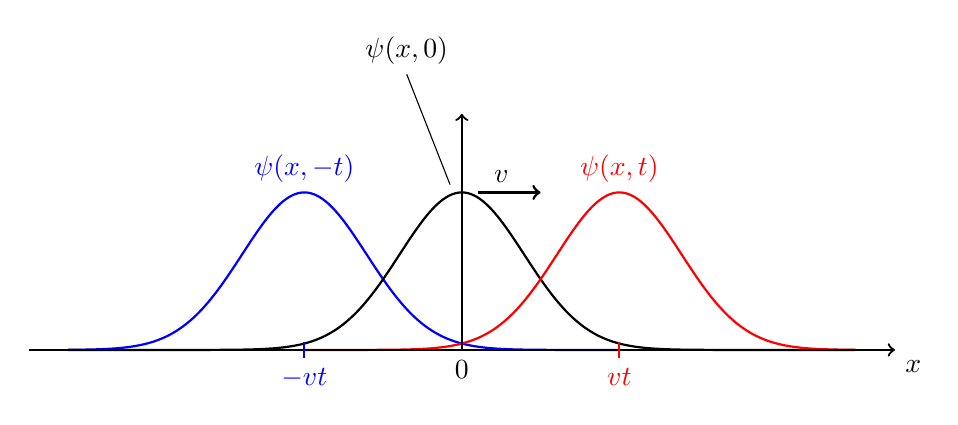
\begin{tikzpicture}
		%rechts
		%\draw[red,line width=1] (4,0) .. controls (3.2,0.2) and (2.8,1.8) .. (2,2);
		%\draw[red,line width=1] (0,0) .. controls (0.8,0.2) and (1.2,1.8) .. (2,2);
		\draw[domain=-5:2, samples=500, blue, thick] plot (\x, {2*exp(-(\x + 2)^(2)*0.8});
		%mitte
		%\draw[line width=1] (-2,0) .. controls (-1.2,0.2) and (-0.8,1.8) .. (0,2);
		%\draw[line width=1] (2,0) .. controls (1.2,0.2) and (0.8,1.8) .. (0,2);
		\draw[domain=-5:5, samples=500, thick] plot (\x, {2*exp(-(\x + 0)^(2)*0.8});
		%links
		%\draw[blue,line width=1] (-4,0) .. controls (-3.2,0.2) and (-2.8,1.8) .. (-2,2);
		%\draw[blue,line width=1] (0,0) .. controls (-0.8,0.2) and (-1.2,1.8) .. (-2,2);
		\draw[domain=-2:5, samples=500, red, thick] plot (\x, {2*exp(-(\x - 2)^(2)*0.8});
		%achsen
		\draw[thick, <-] (5.5,0) node[anchor=north west] {$x$}-- (-5.5,0);
		\draw[thick, ->] (0,0) node[below] {$0$} -- (0,3); % node[anchor=south east] {$y$};
		%
		\draw[line width=1,->] (0.2,2) -- (1,2);
		\draw[dotted] (0.5,2) node[above] {$v$};
		\draw[thick, red] (2,0.1) -- (2,-0.1) node[below] {$vt$};
		\draw[thick, blue] (-2,0.1) -- (-2,-0.1) node[below] {$-vt$};
		\draw[dotted] (2,2) node[red,above] {$\psi (x,t)$};
		\draw[dotted] (-2,2) node[blue,above] {$\psi (x,-t)$};
		\draw (-.7,3.5) node[above] {$\psi (x,0)$} -- (-0.15,2.1);
	\end{tikzpicture}
\end{center}
$ t > 0: \quad \Psi_-(x,t) = f(x - vt) $\\
$ \Psi_+(x,t) = f(x + vt) $\\[5pt]
Wellengleichungen sind linear $ \Rightarrow $ Linearkombinationen von Lösungen sind wieder Lösungen.
\begin{align*}
\Psi(x,t) &= a_1 \Psi_1(x,t) + a_2 \Psi_2(x,t)\\
&= a_1 f_1(x+vt) + a_2 f_2(x-vt)
\end{align*}
\lcom{Im allgemeinen muss es aber nicht sein, dass eine Welle bei Zeittransformationen ihre Form beibehält!}\\
\begin{center}
	%t2:
	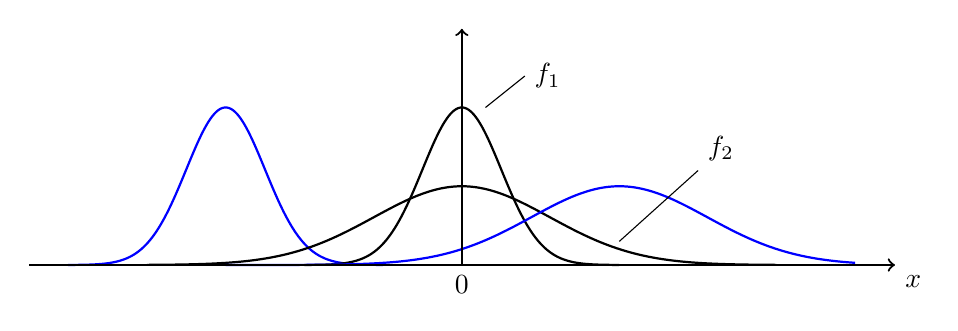
\begin{tikzpicture}
		%\draw[line width=1,blue] (-4.5,0) .. controls (-3.3,0.1) and (-3.8,1.8) .. (-3,2);
		%\draw[line width=1,blue] (-1.5,0) .. controls (-2.7,0.1) and (-2.2,1.8) .. (-3,2);
		\draw[domain=-5:-1, samples=500, blue, thick] plot (\x, {2*exp(-(\x + 3)^(2)*2});
		%
		%\draw[line width=1] (-1.5,0) .. controls (-0.3,0.1) and (-0.8,1.8) .. (0,2);
		%\draw[line width=1] (1.5,0) .. controls (0.3,0.1) and (0.8,1.8) .. (0,2);
		\draw[domain=-2:2, samples=500, thick] plot (\x, {2*exp(-(\x + 0)^(2)*2});
		%
		%\draw[line width=1] (-3.5,0) .. controls (-1.2,0) and (-1.1,0.9) .. (0,1);
		%\draw[line width=1] (3.5,0) .. controls (1.2,0) and (1.1,0.9) .. (0,1);
		\draw[domain=-4:4, samples=500, thick] plot (\x, {1*exp(-(\x + 0)^(2)*.4});
		%
		%\draw[line width=1,blue] (-1.5,0) .. controls (0.8,0) and (0.9,0.9) .. (2,1);
		%\draw[line width=1,blue] (5.5,0) .. controls (3.2,0) and (3.1,0.9) .. (2,1);
		\draw[domain=-3:5, samples=500, blue, thick] plot (\x, {1*exp(-(\x - 2)^(2)*.4});
		%achsen
		\draw[thick, <-] (5.5,0) node[anchor=north west] {$x$}-- (-5.5,0);
		\draw[thick, ->] (0,0) node[below] {$0$} -- (0,3); % node[anchor=south east] {$y$};
		%
		\draw (2,.3) -- (3,1.2) node[anchor=south west] {$f_2$};
		\draw (0.3,2) -- (0.8,2.4) node[right] {$f_1$};
	\end{tikzpicture}
\end{center}
Man kann zeigen, dass die allgemeine Lösung der Wellengleichung in einer Dimension geschrieben werden kann als:
\begin{equation*}
\Psi(x,t) = f(x + vt) + g(x - vt)
\end{equation*}
Besonders Wichtig:\\
\textbf{Ebene Wellen (1D)}
\begin{align*}
\Psi_{\pm}(x,t) &= a \cos(kx \pm \omega t)\\
&= a \cos(k (x \pm \frac{\omega}{k} t))
\end{align*}
$ a \in \mathbb{R} \quad \omega, k \in \mathbb{R} \quad \omega, k > 0 $\\
$ \Psi_\pm $ löst die Wellengleichung:
\begin{equation*}
\prt{^2}{x^2} \Psi - \frac{1}{v^2} \prt{^2 \Psi}{t^2} = 0
\end{equation*}
falls $ \frac{\omega}{k} = v $\\
\begin{minipage}{.5\linewidth}
	\textbf{Dispersionsrelation:}\\
	$ \omega = k v = \omega(k) $\\
	Wellenzahl $ k $, Wellenlänge $ \lambda = \frac{2 \pi}{k} $
\end{minipage}%
\begin{minipage}{.5\linewidth}
	%t3:
	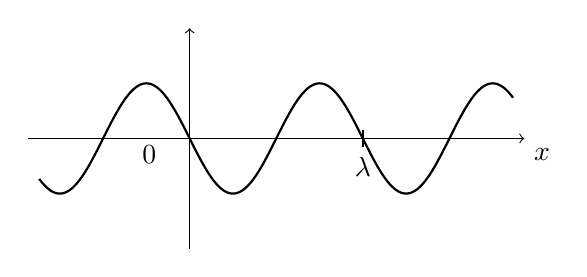
\begin{tikzpicture}[scale=.7]
		\draw[<-] (4.5,0) node[anchor=north west] {$x$}-- (-4.5,0);
		\draw[->] (-pi/2,-2) -- (-pi/2,2); % node[anchor=south east] {$y$};
		\draw[thick,domain=-4.3:4.3, samples=500] plot (\x, {sin(2*\x r)});
		\draw[dotted] (-2,-0.3) node[left] {$0$};
		\draw[thick] (pi/2,0.15) -- (pi/2,-0.15) node[below] {$\lambda$};
	\end{tikzpicture}
\end{minipage}%
\begin{align*}
\Psi_{\pm} (x + n \lambda t) &= a \cos(k (x + n \lambda) \pm \omega t)\\
&= a \cos( k x \pm \omega t + k n \lambda)\\
&= a \cos(kx \pm \omega t) \\
&= \Psi_{\pm} (x,t)
\end{align*}
Die Kreisfrequenz $ \omega $, Frequenz $ \nu = \frac{\omega}{2 \pi} $, Schwingungsdauer $ \tau = \frac{1}{\nu} = \frac{2 \pi}{\omega} $
\begin{align*}
\Psi_{\pm} (x,t + n \tau) &= a \cos( kx \pm \omega(t + n \tau)) = a \cos(kx \pm \omega t \pm n \ub{\omega \tau}_{= 2 \pi}) \quad n \in \mathbb{Z} \\
&= a \cos(kx \pm \omega t) = \Psi_{\pm}(x,t)
\end{align*}
\begin{center}
	%t4:
	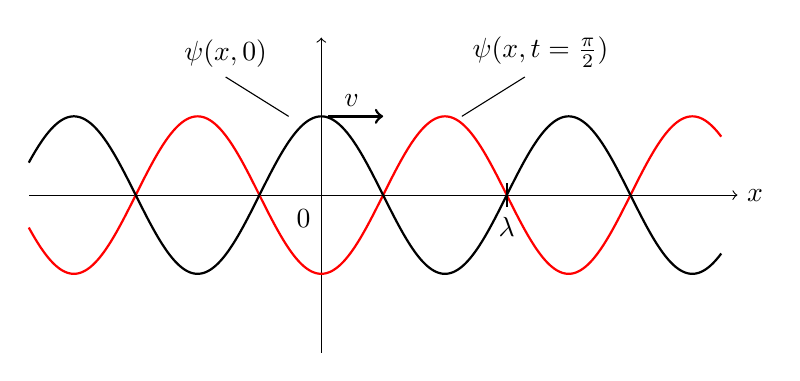
\begin{tikzpicture}
		\draw[<-] (4.5,0) node[right] {$x$}-- (-4.5,0);
		\draw[->] (-pi/4,-2) -- (-pi/4,2); % node[right] {$y$};
		\draw[red,thick,domain=-4.5:4.3, samples=500] plot (\x, {sin(2*\x r)});
		\draw[dotted] (-.8,-0.3) node[left] {$0$};
		\draw[thick] (pi/2,0.15) -- (pi/2,-0.15) node[below] {$\lambda$};
		\draw[thick,domain=-4.5:4.3, samples=500] plot (\x, {-sin(2*\x r)});
		\draw[dotted] (-0.4,1) node[above] {$v$};
		\draw[dotted] (-2,1.5) node[above] {$\psi(x,0)$};
		\draw (-1.2,1) -- (-2,1.5);
		\draw[line width=1,->] (-0.7,1) -- (0,1);
		\draw[dotted] (2,1.5) node[above] {$\psi(x,t=\frac{\pi}{2})$};
		\draw (1,1) -- (1.8,1.5);
	\end{tikzpicture}
\end{center}
Die Phasengeschwindigkeit $ v $:
\begin{equation*}
v = \frac{\omega}{k} = \frac{\lambda}{2 \pi} \omega = \lambda \nu = \frac{\lambda}{\tau}
\end{equation*}
Ebenso wird die Wellengleichung mit einem Sinus gelöst:
\begin{equation*}
\Psi_{\pm} (x,t) = a \sin(kx \pm \omega t)
\end{equation*}
Beide Lösungen sind also enthalten in:
\begin{equation*}
\Psi(x,t) = a e^{i(\ob{kx - \omega t}^{\varphi \tx{ Phase}})}
\end{equation*}
$ a \in \mathbb{C} \quad k \in \mathbb{R} $\\
$ \omega = v |k| $\\
Für Physikalische Felder gilt:
\begin{equation*}
\Psi(x,t) = \Re\left(a e^{i(kx - \omega t)}\right)
\end{equation*}

\subsection{Ebene Wellen in 3 Raumdimensionen}
\begin{equation*}
\Delta \Psi(\vec{r} ,t) - \frac{1}{v^2} \prt{^2 \Psi}{t^2} = 0
\end{equation*}
eben Welle:
\begin{equation*}
\Psi(\vec{r} ,t) = a e^{i (\vec{k} \cdot \vec{r} - \omega t)}
\end{equation*}
Mit dem Wellenvektor:\\
$ \vec{k} = (k_x, k_y, k_z)^\top $\\
und der Frequenz\\
$ \omega \ge 0 $
\begin{align*}
\Delta \Psi &= \left(\prt{^2}{x^2} + \prt{^2}{y^2} + \prt{^2}{z^2}\right) a e^{i(\vec{k} \cdot \vec{r} - \omega t)} \\
&= i^2 (k_x^2 + k_y^2 + k_z^2) a e^{i(\vec{k} \cdot \vec{r} - \omega t)}\\
&= - k^2 \Psi
\end{align*}
\begin{equation*}
\prt{^2 \Psi}{t^2} = - \omega^2 \Psi
\end{equation*}
\begin{equation*}
\Delta \Psi - \frac{1}{v^2} \prt{^2 \Psi}{t^2} = \ob{\left(- k^2 + \frac{\omega^2}{v^2}\right)}^{=0} \Psi = 0
\end{equation*}
$ k^2 = \frac{\omega^2}{v^2} \qquad \omega = v |\vec{k}| $\\[5pt]
\emph{Bemerkung:}\\
\begin{minipage}{.5\linewidth}
	\begin{enumerate}[i)]
		\item ebene Welle:\\
		$ \Psi(\vec{r,t}) $ konstant falls Phase konstant.\\
		$ \varphi (\vec{r} ,t) = \vec{k} \cdot \vec{r} - \omega t = \const $\\
		Für festes $ t $: $ \vec{k} \cdot \vec{r} = \const $
		\item Phasengeschwindigkeit
		\begin{equation*}
		v = \frac{\omega}{|\vec{k}|}
		\end{equation*}
	\end{enumerate}
\end{minipage}%
\begin{minipage}{.5\linewidth}
	\flushright
	%t5:
	\begin{tikzpicture}[scale=.8]
		\draw[->] (0,-1) -- (0,3) node[anchor=south east] {$ y $};
		\draw[->] (-1,0) -- (4.5,0) node[anchor=north west] {$ x $};
		\coordinate (o) at (.5,-1);
		\draw[thick, ->] (o) -- ++(45:4) node[anchor=south west] {$ \vec{x} \  \substack{\tx{Ausbreitungs-} \\ \tx{Richtung}} $ };
		\draw ($ (o) + (135:3) $) -- ++(-45:6);
		\draw ($ (o) + (135:3) + (45:1.5) $) -- ++(-45:6);
		\draw ($ (o) + (135:3) + (45:3) $) -- ++(-45:6);
		\draw[decorate, decoration={brace,amplitude=10pt,raise=18pt}, xshift=2pt, yshift=-2pt]  ($ (o) + (135:2.5) $) -- node[anchor=south east, xshift=-15pt, yshift=15pt] {$\lambda = \frac{2 \pi}{k}$}  ($ (o) + (135:2.5) + (45:1.5) $);
		\draw[thick, <->] ($ (o) + (135:2.5) $) -- ($ (o) + (135:2.5) + (45:1.5) $);
	\end{tikzpicture}
\end{minipage}%
\begin{enumerate}
	\item[iii)] Wellengleichung linear\\
	$ \Rightarrow $ Linearkombinationen von Lösungen sind wieder Lösungen.
	\begin{equation*}
	\Psi(\vec{r},t) = a_1 e^{i(\vec{k}_1 \cdot \vec{r} - \omega_1 t)} + a_2 e^{i(\vec{k}_2 \cdot \vec{r} - \omega_2 t)}
	\end{equation*}
\end{enumerate}
\subsubsection{Allgemeine Lösung der Wellengleichung}
\begin{equation*}
\Psi(\vec{r},t) = \int \dd^3 k a(\vec{k}) e^{i(\vec{k} \cdot \vec{r} - \omega t)}
\end{equation*}
\begin{equation*}
\omega(\vec{k}) = v |\vec{k}|
\end{equation*}

\subsection{Ebene elektromagnetische Wellen}

\begin{equation*}
\Rightarrow \quad \rmbox{\Delta \vec{E} - \frac{1}{v^2} \prt{^2 \vec{E}}{t^2} = 0} \qquad 
\Rightarrow \quad \rmbox{\Delta \vec{B} - \frac{1}{v^2} \prt{^2 \vec{B}}{t^2} = 0}
\end{equation*}
Lösungen:
\begin{equation*}
\vec{E} = \vec{E}_0 e^{i(\vec{k} \cdot \vec{r} - \omega t)} \qquad \vec{B} = \vec{B}_0 e^{i(\tilde{\vec{k}} \cdot \vec{r} - \tilde{\omega} t)}
\end{equation*}
$ \omega = v |\vec{k}| \quad \tilde{\omega} = v |\tilde{\vec{k}}| \quad \vec{k}, \tilde{\vec{k}} \in \mathbb{R}^3 $
\begin{enumerate}[i)]
	\item $ \vabla \times \vec{E} = - \prt{\vec{B}}{t} $
	\begin{equation*}
	i (\vec{k} \times \vec{E}_0) e^{i(\vec{k} \cdot \vec{r} - \omega t)} = i \tilde{\omega} \vec{B}_0 e^{i(\tilde{\vec{k}} \cdot \vec{r} - \tilde\omega t)} \qquad \forall \vec{r},t
	\end{equation*}
	$ \Rightarrow \tilde{\vec{k}} = \vec{k} \quad \tilde{\omega} = \omega $\\
	$ \Rightarrow \vec{k} \times \vec{E}_0 = \omega \vec{B}_0 \ \rightarrow \ \vec{B}_0 = \frac{1}{\omega} \vec{k} \times \vec{E}_0 $
	$$\vec{B} \perp \vec{k}, \vec{E}$$
	$$ \Rightarrow \vec{B} = \frac{1}{\omega} \vec{k} \times \vec{E} $$
	\item $ \vabla \times \vec{E} = 0 $
	\begin{align*}
	0 &= \vabla \cdot \vec{E}_0 e^{i(\vec{k} \cdot \vec{r} - \omega t)}\\
	&= i(\vec{k} \cdot \vec{E}_0) e^{i(\vec{k} \cdot \vec{r} - \omega t)}
	\end{align*}
	$ \Rightarrow \vec{k} \cdot \vec{E}_0 \ \rightarrow \ \vec{k} \cdot \vec{E}_0 = 0 $
	$$ \vec{k} \perp \vec{E} $$
	\item $ \vabla \cdot \vec{B} = 0 $\\
	$ \Rightarrow \vec{k} \cdot \vec{B}_0 = 0 \Rightarrow \vec{k} \cdot \vec{B} = 0 $
	\item $ \vabla \times \vec{B} = \frac{1}{v^2} \prt{\vec{E}}{t} $\\
	$ \Rightarrow i \vec{k} \times \vec{B}_0 = - i \frac{1}{v^2} \omega \vec{E}_0 $\\
	$ \Rightarrow \vec{k} \times \vec{B}_0 = - \frac{\omega}{v^2} \vec{E}_0 $\\
	$ \Rightarrow \vec{E} = -\frac{v^2}{\omega} \vec{k} \times \vec{B} $
\end{enumerate}
\begin{minipage}{.5\linewidth}
	$ \vec{E}, \vec{B}, \vec{k} $ orthogonal zueinander\\
	$ \Rightarrow $ transversale Welle\\
	Beziehung zwischen der Amplitude von $ \vec{B}, \vec{E} $:
	\begin{equation*}
	|\vec{B}| = \frac{1}{\omega} |\vec{k} \times \vec{E}| = \frac{|\vec{k}|}{\omega} |\vec{E}| = \frac{1}{v} |\vec{E}|
	\end{equation*}
\end{minipage}%
\begin{minipage}{.5\linewidth}
	\flushright
	%t6:
	\begin{tikzpicture}
		\draw[thick,->] (0,0) -- (0,1.5) node[anchor=south east] {$ \vec{E} $};
		\draw[thick,->] (0,0) -- (1.5,0) node[anchor=north west] {$ \vec{S} $};
		\draw[thick,->] (0,0) -- (-.75,-.75) node[anchor=north east] {$ \vec{B} $};
	\end{tikzpicture}
\end{minipage}%
\\
o.B.d.A. $ \quad \vec{k} = k \vec{e}_z $
\begin{align*}
\vec{E} &= (E_{0_x} \vec{e}_x + E_{0_y} \vec{e}_y) e^{i(k \cdot r - \omega t)} \\
\vec{B} &= \frac{1}{\omega} \vec{k} \times \vec{E} = \frac{k}{\omega} \vec{e}_z \times (E_{0_x} \vec{e}_x + E_{0_y} \vec{e}_y) e^{i(k \cdot r - \omega t)} \\
&= \frac{1}{v} (- E_{0_y} \vec{e}_x + E_{0_x} \vec{e}_y) e^{i(k \cdot r - \omega t)} 
\end{align*}
i.A. $ E_{0_x}, E_{0_y} \in \mathbb{C} $
\begin{equation*}
\vec{E} = \Re\left(\vec{E}_0 e^{i(k \cdot r - \omega t)} \right)
\end{equation*}
\emph{Beispiel:} $ E_{0_y} = 0 \quad E_{0_x} \in \mathbb{R} $
\begin{align}
\vec{E} &= E_{0_x} \cos (kz - \omega t) \vec{e}_x \\
\vec{B} &= \frac{E_{0_x}}{v} \cos(kz - \omega t) \vec{e}_y
\end{align}

%t7: (EM-Welle Tikz): (v in ausbreitungs richtung einzeichnen)
\begin{center}
	%t3:
	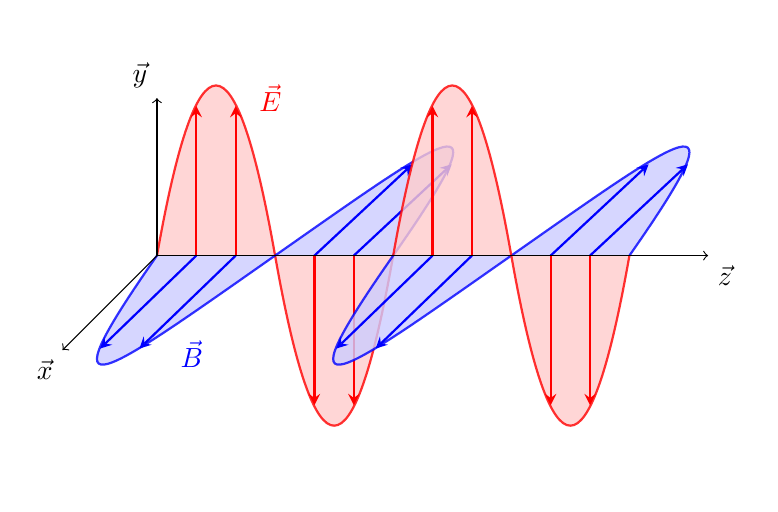
\begin{tikzpicture}%[>=stealth]
	% E
	\draw[red,thick,looseness=5,fill=red!20!white,opacity=.8] (0,0) to[out=80,in=100] (1.5,0) to[out=-80,in=-100] (3,0);
	\foreach \z in {.5,1}
	\draw[thick,red,->,>=stealth] (\z,0) -- ++(0,1.9);
	\foreach \z in {2,2.5}
	\draw[thick,red,->,>=stealth] (\z,0) -- ++(0,-1.9);
	% B
	\draw[blue,thick,looseness=4.5,fill=blue!20!white,opacity=.8] (0,0) to[out=-125,in=-145] (1.5,0) to[out=35,in=55] (3,0) to[out=-125,in=-145] (4.5,0) to[out=35,in=55] (6,0);
	\foreach \z in {.5,1,3.5,4}
	\draw[thick,blue,->,>=stealth] (\z,0) -- ++(-136:1.7cm);
	\foreach \z in {2,2.5,5,5.5}
	\draw[thick,blue,->,>=stealth] (\z,0) -- ++(43:1.7cm);
	% rest E
	\draw[red,thick,looseness=5,fill=red!20!white,opacity=.8] (3,0) to[out=80,in=100] (4.5,0) to[out=-80,in=-100] (6,0);
	\foreach \z in {3.5,4}
	\draw[thick,red,->,>=stealth] (\z,0) -- ++(0,1.9);
	\foreach \z in {5,5.5}
	\draw[thick,red,->,>=stealth] (\z,0) -- ++(0,-1.9);
	% koordinatensystem
	\draw[->] (0,0) -- (0,2) node[anchor=south east] {$ \vec{y} $};
	\draw[->] (0,0) -- (-1.2,-1.2) node[anchor=north east] {$ \vec{x} $};
	\draw[->] (0,0) -- (7,0) node[anchor=north west] {$ \vec{z} $};
	\node (e) at (1.5,2) {\color{red} $ \vec{E} $ \color{black}};
	\node (b) at (.5,-1.25) {\color{blue} $ \vec{B} $ \color{black}};
	\end{tikzpicture}
\end{center}

\subsection{Polarisation ebener EM-Wellen}

Charakterisierung der Schwingungsrichtung $ \vec{k} = k \vec{e}_z $
\begin{equation*}
\vec{E} = (E_{0_x} \vec{e}_x + E_{0_y} \vec{e}_y) e^{i(kx - \omega t)}
\end{equation*}
\begin{equation*}
E_{0_x} = |E_{0_x} e^{i \varphi} \qquad E_{0_y} = |E_{0_y} e^{i (\varphi + \delta)}
\end{equation*}
Physikalisches Feld:
\begin{align*}
\vec{E} &= \Re \left[ (E_{0_x} \vec{e}_x + E_{0_y} \vec{e}_y) e^{i(k \cdot r - \omega t)} \right]\\
&= |E_{0_x}| \cos(kz - \omega t + \varphi) \vec{e}_x + |E_{0_y}| \cos(kz - \omega t + \varphi + \delta) \vec{e}_y
\end{align*}
\textbf{Fälle:}\\
\begin{enumerate}[i)]
	\item
	$ \delta = 0 $ oder $ \delta = \pm \pi $
	\begin{equation*}
	\Rightarrow \quad \vec{E} = \ub{(|E_{0_x} \vec{e}_x \pm |E_{0_y} \vec{e}_y)}_{\mathclap{\substack{\tx{orts- und} \\ \tx{Zeitunabh.}}}} \cos(kz - \omega t)
	\end{equation*}
	$ \rightarrow \vec{E} $ schwingt in fester Richtung! Die \textbf{Polarisationsrichtung}
	$ \rightarrow $ \textbf{linear Polarisiert}
	\item
	$ \delta = \pm \frac{\pi}{2} \quad |E_{0_x}| = |E_{0_y}| = E $
	\textbf{Zirkulär Polarisiert}
	\begin{align*}
	\vec{E} = E\ub{(\vec{e}_x \cos(kz - \omega t + \varphi)) \mp \vec{e}_y \sin(kz - \omega t + \varphi))}_{ = \vec{r} (t)}
	\end{align*}
	\lcom{$ |\vec{r}| = 1 $ und $ \vec{r} $ läuft mit $ \omega $ um}
	\item
	$ \delta , |E_{0_x}|, |E_{0_y}| $ beliebig:
	\textbf{elliptisch Polarisiert}
\end{enumerate}
\begin{center}
	%t8:
	\begin{tikzpicture}
		\draw[->] (0,-2) -- (0,2) node[anchor=south east] {$ y $};
		\draw[->] (-2,0) -- (2,0) node[anchor=north west] {$ x $};
		\draw[thick,->] (0,0) -- (1.2,1.2) node[anchor=south west] {$ \vec{E} $};
		\draw[->] (0,0) -- (-1.2,-1.2);
		\draw[thick] ($ (1.2,0) + (0,.15) $) -- ++(0,-.3) node[below] {$ |E_{0_x}| $};
		\draw[thick] ($ (0,1.2) + (.15,0) $) -- ++(-.3,0) node[left] {$ |E_{0_y}| $};
		%
		\draw[white] (2,-2) -- ++(0,-.225);
	\end{tikzpicture}%
	%t9:
	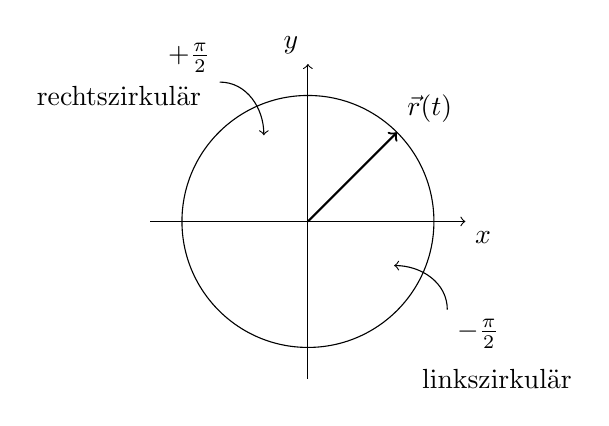
\begin{tikzpicture}[scale=.8]
		\draw[->] (0,-2.5) -- (0,2.5) node[anchor=south east] {$ y $};
		\draw[->] (-2.5,0) -- (2.5,0) node[anchor=north west] {$ x $};
		\draw[thick,->] (0,0) -- ({cos(45) * 2}, {sin(45) * 2}) node[anchor=south west] {$ \vec{r}(t) $};
		\draw (0,0) circle (2cm);
		\centerarc[thick, <->](0,0)(120:-30:1.2);
		\node (a) at (-30:1.4) {};
		\draw[<-] (a) to[out=0,in=90] ++(1,-.7) node[anchor=north west] {$ - \frac{\pi}{2} $};
		\node at (-3,2) {rechtszirkulär};
		\node (b) at (120:1.4) {};
		\draw[<-] (b) to[out=90,in=0] ++(-.7,1) node[anchor=south east] {$ + \frac{\pi}{2} $};
		\node at (3,-2.5) {linkszirkulär};
	\end{tikzpicture}%
	%t10:
	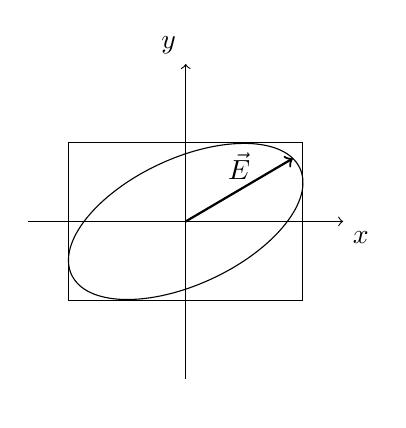
\begin{tikzpicture}[scale=.8]
		\draw[->] (0,-2.5) -- (0,2.5) node[anchor=south east] {$ y $};
		\draw[->] (-2.5,0) -- (2.5,0) node[anchor=north west] {$ x $};
		\draw[rotate=25] (0,0) ellipse (2cm and 1cm);
		\draw (-1.86,-1.25) rectangle (1.86,1.25);
		\draw[thick, ->] (0,0) -- node[above] {$ \vec{E} $} (1.7,1); %({cos(25) * 2},{sin(25) * 2});
		%
		\draw[white] (2,-2.5) -- ++(0,-0.315);
	\end{tikzpicture}
\end{center}